\documentclass[a4paper,12pt]{article}
\linespread{1.15}
\usepackage{tma}
\usepackage{amsmath}
\usepackage{siunitx}
\newcommand{\Mod}[1]{\ (\mathrm{mod}\ #1)}
\usepackage{tikz}
\newcommand*\circled[1]{\tikz[baseline=(char.base)]{
            \node[shape=circle,draw,inner sep=2pt] (char) {#1};}}

\mypin{student: 23092186}
\mycourse{COMP0080 - CW2}

%\marginnotes

\begin{document}
\section*{2 LDPC codes}
\begin{enumerate}
\item[(2.2.1)]
Question: Print the outputs of the function for the matrix.\\
Answer: For the given parity check matrix $H$ \\

 \[
H = \begin{bmatrix}
    1 & 1 & 1 & 1 & 0 & 0 \\
    0 & 0 & 1 & 1 & 0 & 1 \\
    1 & 0 & 0 & 1 & 1 & 0
\end{bmatrix}
\]

The systematic form of this $H$, $\hat{H}$ is:

\[
\hat{H} = \begin{bmatrix}
    1 & 0 & 0 & 1 & 1 & 1 \\
    0 & 1 & 0 & 0 & 1 & 1 \\
    0 & 0 & 1 & 1 & 0 & 1
\end{bmatrix}
\]

The systematic encoding matrix of this $H$, ${G}$ is:\\
 
 \[
G = \begin{bmatrix}
    1 & 1 & 1 \\
    0 & 1 & 1 \\
    1 & 0 & 1 \\
    1 & 0 & 0 \\
    0 & 1 & 0 \\
    0 & 0 & 1 \\
\end{bmatrix}
\]

\item[(2.2.2)] Question: Draw a factor-graph for the parity check matrix $H$ shown in question 2.2.1: \\
Answer: The 3 factors $f1$, $f2$ and $f3$, each corresponding to a parity check (i.e. the 3 rows of the parity check matrix $H$) are shown in squares as is the convention. \\
The edges connecting each factor to specific variables ($x1$, $x2$, $x3$, $x4$, $x5$, $x6$ ) indicate which variables of the input vector $X$ are involved in the constraint of a given factor. \\
So for $f1$, the first four variables should sum to 0 because the first four bits along the first row are 1, the last two are 0, and so on.\\

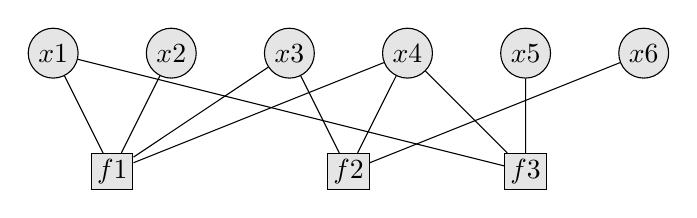
\begin{tikzpicture}[scale=1.5, auto,swap]
  
    \foreach \pos/\name in {{(0,2)/x1}, {(1,2)/x2}, {(2,2)/x3}, {(3,2)/x4}, {(4,2)/x5}, {(5,2)/x6}}
        \node[circle, draw, inner sep=2pt, fill=gray!20] (\name) at \pos {$\name$};
    
    \foreach \pos/\name in {{(0.5,1)/f1}, {(2.5,1)/f2}, {(4,1)/f3}}
        \node[rectangle, draw, inner sep=2pt, fill=gray!20] (\name) at \pos {$\name$};
    
    \draw (x1) -- (f1);
    \draw (x2) -- (f1);
    \draw (x3) -- (f1);
    \draw (x3) -- (f2);
    \draw (x4) -- (f1);
    \draw (x4) -- (f2);
    \draw (x4) -- (f3);
    \draw (x6) -- (f2);
    \draw (x1) -- (f3);
    \draw (x5) -- (f3);
\end{tikzpicture}
\end{enumerate}
\clearpage

\section*{2 LDPC codes contin.}
\begin{enumerate}
\item[(2.2.2)] 
Question: Write the distribution corresponding to this factor-graph and the updates used for the messages.\\
Answer: The probability distribution of the constraints defined by $H$ from 2.2.1. are three conditionally-independent joint distributions, so the whole distribution is their product:\\
$p(x_1, x_2, x_3, x_4) \times p(x_3, x_4, x_6) \times p(x_1, x_4, x_5)$

The updates of the values used for the messages occurs in steps 2 and 3 (from the slides), (with step 1 as the initialisation and step 4 as the evaluation of whether we have reached convergence).\\
Step 2 involves recomputing (hence updating) factor-to-variable messages:

$\mu_{f_m \rightarrow \text{x}_n}(\text{x}_n) = \sum\limits_{\text{x}_{n'}, n' \in N(m) \backslash n} \left[ I\left[\text{x}_n + \sum\limits_{n'} \text{x}_{n'} = 0\right] \right] \prod\limits_{\text{x}_{n'}, n' \in N(m) \backslash n} \mu_{\text{x}_{n'} \rightarrow f_m}(\text{x}_{n'})$\\\\

Step 3 involves recomputing (hence updating) variable-to-factor messages:

$\mu_{\text{x}_n \rightarrow f_m} \propto p(\text{y}_n|\text{x}_n) \prod\limits_{m' \in N(n) \backslash m} \mu_{f_{m'} \rightarrow \text{x}_n}(\text{x}_n)$\\

\end{enumerate}
\clearpage
\section*{2 LDPC codes contin.}
\begin{enumerate}
\item[(2.2.3)] Question: Print the result of the decoding for a given parity check matrix $H_1$ and vector $y_1$.

Answer: The Python script `ldpc.py` has been written to adhere as much as possible to the description in the ldpc slides and talks. It is well documented and written to be readable in an object-oriented format. Unfortunately though it is not optimised and seems to be not possible to run to completion on a laptop, which becomes overheated. As such, it has not been possible to decode the vector $y1$.
\item[(2.2.4)] Question: Recover the original English message.
Answer: NA
\end{enumerate}

\clearpage
\end{document}